\chapter{Governing Equations for Oxygen Transport}
\label{ch:o2equations}

\section{Species conservation equation}

Let $C(\vect x,t)$ be the molar concentration of dissolved oxygen. A balance on a fixed control volume, with the molar flux $\vect J=C\vect u-D\nabla C$ (convection plus Fickian diffusion \citep{BSL2002,Deen2012}), gives
\begin{equation}
\underbrace{\frac{\partial C}{\partial t}}_{\text{accumulation}}
+\underbrace{\nabla\cdot(\vect uC)}_{\text{convection}}
=\underbrace{\nabla\cdot(D\nabla C)}_{\text{diffusion}}
+\underbrace{R}_{\text{volumetric production}} .
\label{eq:ox_general}
\end{equation}
\begin{itemize}
\item The accumulation term is the rate of change of oxygen stored in a unit volume.
\item The convective term is the net outflow of oxygen carried by the medium.
\item The diffusive term is the net inflow by molecular diffusion down concentration gradients, with diffusivity $D$.
\item $R$ (\si{mol.m^{-3}.s^{-1}}) is the production rate per unit volume; consumption is negative.
\end{itemize}

\section{Simplification of the governing equation}

Each assumption below is checked against the actual parameters (\cref{tab:o2params}). The list states whether an assumption is \emph{used} in the model or is only an alternative.

\begin{enumerate}
\item \textbf{Dilute solution} (used). The oxygen mass fraction is $Y=CM_{\mathrm{O_2}}/\rho=0.178\times0.032/981.8\approx\num{5.8e-6}$. Oxygen therefore has no effect on the density or viscosity of the medium, and Fick's law for a dilute binary mixture applies.
\item \textbf{Constant diffusivity} (used). The system is isothermal at \SI{37}{\celsius}, so $D=\SI{3.0e-9}{m^2/s}$ \citep{HanBartels1996}, with a sensitivity range of 2.6--\SI{3.3e-9}{m^2/s}. Then $\nabla\cdot(D\nabla C)=D\nabla^2C$.
\item \textbf{Incompressible flow} (used). Since $\nabla\cdot\vect u=0$ (\cref{eq:gov_cont}), $\nabla\cdot(\vect uC)=\vect u\cdot\nabla C$.
\item \textbf{One-way coupling} (used). Oxygen does not affect the flow (point 1), so the velocity field of Part A is prescribed (``frozen'').
\item \textbf{No reaction in the medium} (used). The medium does not consume oxygen, so $R=0$ in the fluid.
\item \textbf{Uptake as a surface flux} (used). A confluent monolayer is about 5--\SI{10}{\micro\metre} thick, much thinner than the gap. The oxygen drop that diffusion through a layer of thickness $\delta_c$ needs to supply the uptake is of order $\qmax\delta_c/D$, i.e.\ a fraction $\Da_w\,\delta_c/h\approx10^{-3}$ of $\Csat$ (with $\Da_w$ defined in \cref{tab:o2groups}). The monolayer can therefore be represented by a boundary flux on the floor. The alternative, a volumetric sink in a layer of thickness $\delta_c$, gives the same result to this accuracy and would require meshing the cell layer.
\item \textbf{Steady state} (used). Three time scales are relevant:
\begin{itemize}
\item diffusion across the gap, $t_D=h^2/D=\SI{7.0}{s}$;
\item residence in the cell-culture section, $t_{\mathrm{res}}=A_{\mathrm{cells}}h/Q=\SI{4553}{s}$, \SI{1002}{s} and \SI{8.3}{s} at 0.22, 1 and \SI{120}{\uLmin};
\item equilibration of the \SI{5}{mm} PDMS lid, of order hours.
\end{itemize}
Cultures last days (5 days to confluence in the reference protocol \citep{Delon2020}), so the steady state is the relevant one. Transients after a medium change or a change of flow rate last up to about 1--\SI{2}{h}, and are outside the scope of this report.
\item \textbf{Uptake kinetics} (Michaelis--Menten used; zero order used for closed forms). Three standard forms are considered:
\begin{equation}
q=\begin{cases}
\qmax & \text{zero order},\\[2pt]
\dfrac{\qmax}{\Km}\,C & \text{first order},\\[6pt]
\qmax\dfrac{C}{\Km+C} & \text{Michaelis--Menten}.
\end{cases}
\label{eq:ox_kinetics}
\end{equation}
Michaelis--Menten kinetics reduces to zero order for $C\gg\Km$ and to first order for $C\ll\Km$. With $\Csat/\Km=283$, the uptake stays within \SI{10}{\percent} of $\qmax$ until $C$ falls below $9\Km\approx0.03\,\Csat$. The zero-order closed forms are therefore accurate wherever the cells are not already close to anoxia. First-order kinetics alone would grossly under-predict the uptake at normal concentrations, so it is used only in the analysis near anoxia.
\end{enumerate}

With these assumptions \cref{eq:ox_general} becomes the steady convection--diffusion equation with a prescribed velocity field,
\begin{equation}
\vect u\cdot\nabla C=D\nabla^2C\qquad\text{in the fluid},
\label{eq:ox_cd}
\end{equation}
and all consumption enters through the boundary condition on the floor.

\section{Coupling with the flow field}

The velocity in \cref{eq:ox_cd} is the steady field validated in \cref{ch:validation}. Two levels of coupling are possible.
\begin{enumerate}
\item \textbf{CFD (planned).} Solve \cref{eq:ox_cd} in Fluent as a user-defined scalar (UDS) on the converged, frozen velocity field, with a user-defined function (UDF) for the Michaelis--Menten wall flux and for the PDMS Robin condition. This set-up has been prepared but not yet run. It would resolve the side-wall layers and the outlet corner.
\item \textbf{Reduced-order model (used here).} Represent the velocity by the lubrication solution validated in Part A: the profile across the gap is parabolic and the flow rate is $Q$ through every section. The oxygen balance then depends only on $Q$, $h$ and $w(x)$. It does not depend on the absolute magnitude of the CFD shear, so the \SI{-5}{\percent} offset of \cref{sec:val_offset} does not affect it.
\end{enumerate}
Both approaches are one-way coupled. Their main limitation is that the reduced-order model treats the cross-section as uniform across the width. The slower fluid in the side-wall layers (about \SI{0.13}{mm} on each side) has a longer residence time and will be more depleted than the reduced-order model predicts. This is a three-dimensional effect that only the CFD can quantify.

\section{Boundary conditions}

The outward unit normal is $\vect n$. The diffusive flux of oxygen into the fluid through a wall is $D\,\partial C/\partial n_{\mathrm{in}}$, where $n_{\mathrm{in}}$ is the inward normal.

\paragraph{Inlet.} $C=\Csat$. The medium arrives equilibrated with the incubator atmosphere: the reservoir and tubing are in the incubator \citep{Delon2020}, and the lead-in is too short for significant uptake. With $\alpha=1.26~\mu\mathrm{M\,mmHg^{-1}}$ and an oxygen partial pressure of \SI{141}{mmHg} in a humidified \SI{5}{\percent} CO$_2$ incubator \citep{Wenger2015}, $\Csat=\SI{0.178}{mol/m^3}$.

\paragraph{Outlet.} Zero diffusive flux, $\partial C/\partial x=0$. Axial diffusion is negligible ($\Pe_L\ge421$, \cref{tab:o2groups}), so the outlet condition has no influence upstream.

\paragraph{Floor (cells), $z=0$.} The cells remove oxygen at the rate $q$:
\begin{equation}
D\left.\frac{\partial C}{\partial z}\right|_{z=0}=q(\Cbot)=\qmax\frac{\Cbot}{\Km+\Cbot},
\label{eq:ox_bc_floor}
\end{equation}
where $\Cbot$ is the local concentration on the floor. This is a non-linear condition: the uptake decreases smoothly when oxygen runs out, instead of driving $C$ negative as a zero-order flux would.

\paragraph{Lid, $z=h$.} Three cases bracket the real device:
\begin{align}
\text{IMP (impermeable):}&\quad \left.\frac{\partial C}{\partial z}\right|_{z=h}=0, \label{eq:ox_bc_imp}\\
\text{PDMS (Robin):}&\quad D\left.\frac{\partial C}{\partial z}\right|_{z=h}=\kp\,(\Csat-\Ctop), \label{eq:ox_bc_pdms}\\
\text{SAT (saturated):}&\quad C(z=h)=\Csat. \label{eq:ox_bc_sat}
\end{align}
IMP is the worst case and represents glass or thermoplastic chips. SAT is the best case, a lid with no transport resistance.

\paragraph{Derivation of the PDMS coefficient.} At steady state, oxygen diffuses through the lid of thickness $t_{\mathrm{PDMS}}$ from incubator air (partial pressure $p_a$) to the PDMS--medium interface (partial pressure $p_i$). With the permeability $P$ (\si{mol.m^{-1}.s^{-1}.Pa^{-1}}) of PDMS, the flux is $N=P(p_a-p_i)/t_{\mathrm{PDMS}}$. Partial pressure is continuous across the interface, and on the medium side Henry's law gives $p_i=\Ctop/\alpha$ and $p_a=\Csat/\alpha$. Hence
\begin{equation}
\begin{aligned}
N&=\frac{P}{t_{\mathrm{PDMS}}\,\alpha}(\Csat-\Ctop)\equiv\kp(\Csat-\Ctop),\\
\kp&=\frac{\num{2.67e-13}}{\num{5e-3}\times\num{9.45e-6}}=\SI{5.65e-6}{m/s},
\end{aligned}
\label{eq:ox_kpdms}
\end{equation}
using $P=800$ Barrer \citep{Merkel2000}. Formulating the condition in partial pressure avoids the partition coefficient between PDMS and medium. The condition assumes that the outer PDMS surface is exposed to incubator air. The reference protocol mentions immersing the device in water to limit bubbles \citep{Delon2020}; this would add a diffusion resistance and lower $\kp$. Reported reductions of PDMS permeability by protein adsorption \citep{Mehta2007} would do the same.

\paragraph{Side walls.} In the CFD the side walls are PDMS and carry the same condition as the lid. The reduced-order model neglects them. Their area per unit length, $2h$, is \SI{29}{\percent} of the floor width at the inlet and less than \SI{3}{\percent} at S5. Neglecting them is therefore conservative for the PDMS case and exact for IMP.

\section{Parameters and dimensionless groups}

\begin{table}[htbp]
\centering
\caption{Oxygen transport parameters. ``Illustrative'' values are not measured data for Caco-2 or A549 cells and are varied in the sensitivity analysis.}
\label{tab:o2params}
\small
\begin{tabularx}{\linewidth}{@{}p{0.22\linewidth}p{0.17\linewidth}p{0.15\linewidth}X@{}}
\toprule
Parameter & Baseline & Range & Source and status\\
\midrule
$D$, O$_2$ in medium, \SI{37}{\celsius} & \SI{3.0e-9}{m^2/s} & 2.6--\SI{3.3e-9}{} & water value \citep{HanBartels1996}; medium taken as water-like\\
$\Csat$ & \SI{0.178}{mol/m^3} & 0.167--0.200 & $1.26~\mu\mathrm{M\,mmHg^{-1}}\times141~\mathrm{mmHg}$ \citep{Wenger2015}\\
Cell density $\rho_{\mathrm{cell}}$ & \SI{2e9}{m^{-2}} & 1--\SI{5e9}{} & seeding density for Caco-2 \tagP\ \citep{Delon2020}; confluent density is higher\\
OCR per cell & \SI{20}{amol/s} & 5--100 & \textbf{illustrative}; mammalian cells span $<1$ to $>350$ \citep{Wagner2011}\\
$\qmax=\rho_{\mathrm{cell}}\cdot$OCR & \SI{4.0e-8}{mol.m^{-2}.s^{-1}} & 0.5--\SI{50e-8}{} & derived (illustrative)\\
$\Km$ & \SI{6.3e-4}{mol/m^3} (\SI{0.5}{mmHg}) & 0.5--\SI{5}{mmHg} & hepatocyte value \citep{Rotem1994}; not cell-line specific\\
PDMS permeability $P$ & 800 Barrer & 600--800 & \citep{Merkel2000}, \SI{35}{\celsius}\\
PDMS thickness & \SI{5}{mm} & -- & \tagP\ \citep{Delon2020}\\
$\kp$ & \SI{5.65e-6}{m/s} & 0 to $\infty$ & derived, \cref{eq:ox_kpdms}\\
\bottomrule
\end{tabularx}
\end{table}

\begin{table}[htbp]
\centering
\caption{Dimensionless groups and time scales of oxygen transport (baseline parameters; $\bar U_0=Q/(w_1h)$ at the inlet of the hyperbola; $A_{\mathrm{cells}}=\SI{115.13}{mm^2}$) \tagM.}
\label{tab:o2groups}
\small
\resizebox{\linewidth}{!}{%
\begin{tabular}{@{}lp{0.37\linewidth}ccc@{}}
\toprule
Group & Meaning & \SI{0.22}{\uLmin} & \SI{1}{\uLmin} & \SI{120}{\uLmin}\\
\midrule
$\Pe_h=\bar U_0h/D$ & convection along $x$ vs diffusion across $h$ & 1.22 & 5.56 & 667\\
$\Pe_L=\bar U_0L/D$ & axial convection vs axial diffusion & 421 & 1916 & \num{2.3e5}\\
$\Da_w=\qmax h/(D\Csat)$ & uptake vs diffusion across the gap & 0.011 & 0.011 & 0.011\\
$\Da_{\mathrm{conv}}=\qmax A_{\mathrm{cells}}/(Q\Csat)$ & total uptake vs convective supply & \textbf{7.06} & \textbf{1.55} & 0.013\\
$\Bi=\kp h/D$ & lid conductance vs gap conductance & 0.27 & 0.27 & 0.27\\
$\Phi_{\mathrm{PDMS}}=\kp\Csat/\qmax$ & maximum lid supply vs maximum uptake & 25.1 & 25.1 & 25.1\\
$\Csat/\Km$ & saturation of the kinetics & 283 & 283 & 283\\
$t_D=h^2/D$ [s] & diffusion time across the gap & 7.0 & 7.0 & 7.0\\
$t_{\mathrm{res}}=A_{\mathrm{cells}}h/Q$ [s] & residence time in the culture section & 4553 & 1002 & 8.3\\
\bottomrule
\end{tabular}}
\end{table}

\Cref{tab:o2groups} and \cref{fig:o2groups} summarise the transport regime.
\begin{itemize}
\item $\Da_w=0.011\ll1$: diffusion across the gap is fast compared with uptake, so the concentration varies by only about \SI{1}{\percent} across the gap.
\item $\Pe_L\gg1$: axial diffusion is negligible.
\item $\Da_{\mathrm{conv}}$ is the decisive group. It exceeds 1 at 0.22 and \SI{1}{\uLmin}: at full uptake the cells would consume more oxygen than the flow brings in. Unless the walls supply the difference, part of the floor must become anoxic.
\item $\Phi_{\mathrm{PDMS}}=25$: a \SI{5}{mm} PDMS lid can supply 25 times the maximum uptake.
\item $t_D/t_{\mathrm{res}}\ll1$ at the two culture flow rates: oxygen equilibrates across the gap long before the medium leaves.
\end{itemize}

\begin{figure}[htbp]
\centering
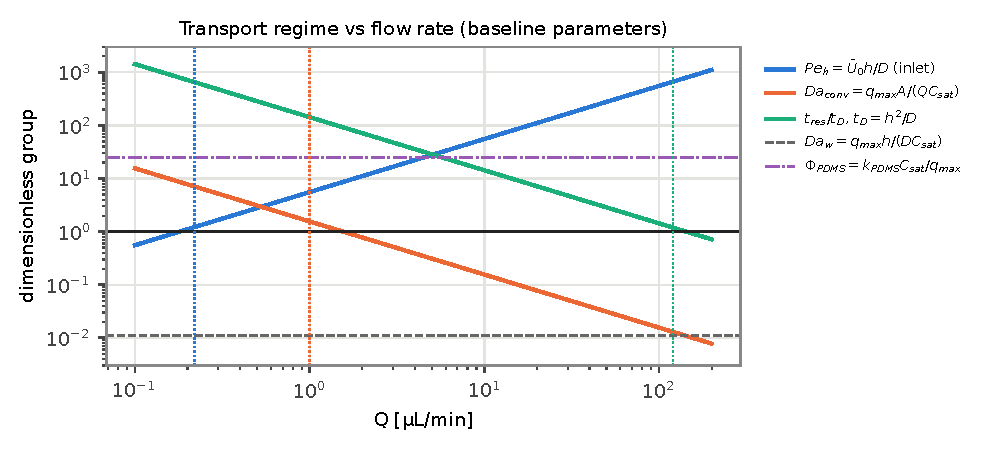
\includegraphics[width=0.9\linewidth]{oxygen_dimensionless_groups.pdf}
\caption{Oxygen transport groups against flow rate (baseline parameters) \tagM. The vertical lines mark the three simulated flow rates. Convection alone can feed the cells only where $\Da_{\mathrm{conv}}<1$, i.e.\ above \SI{1.55}{\uLmin}.}
\label{fig:o2groups}
\end{figure}
